%在实际应用中，oos 经常碰到，所以重要，
%由于OOS 训练见不到，现有方法缺点，1\不灵活 ，2、设置阈值，3、模型复杂
% in this paper 我们的贡献，不做人和假设，可以apply到任何分部，
%引入合成的outlier， hard sample， general的sample起什么作用， 非常容易获取
%Intent detection aims at distinguishing user input utterances to provide corresponding downstream services and is one of the core components of task-oriented dialogue systems. 
% However, the set of user utterances is usually unlimited large in practical while dialogue systems can only support a small set of intent classes. 
%However, in practical, it is a common situation that the user utterances are not in the supported intent set.
% Therefore, it is important to detect out-of-scope (OOS) utterances while correctly distinguish supported intent classes.
%Since OOS utterances can be generally anything that the user wants to input into the dialogue system, it is hard to define OOS utterances and collect OOS examples for training.
%To train models without OOS examples, previous approaches usually adopt clustering methods which are heavily rely on strong assumptions about intent distribution such as Gaussian distributions to build effective decision boundaries, resulting in either complex multi-step training procedure or human-dependent interference during inference such as confidence threshold selection for OOS utterances.
%In this paper, we propose an effective yet simple algorithm to train an OOS intent detection model in a fully end-to-end manner. We follow the truth that OOS utterances can be anything and give no assumption on intent distribution. This advantage makes our method can be applied to any intent system at any scale. 
%We explicitly introduce the supervision information about OOS utterances during training by forming an OOS training set.
%We define the OOS utterances into a hard set and a simple set. The hard OOS utterances stand for the utterances that highly resemble supported intents whereas the simple utterances stand for the utterances that have distinctive different semantic meanings than supported intents. 
%Specifically, we generate hard OOS utterances by forming random convex combinations between embedded labeled utterances from different intent classes. And the simple utterances are sentences extracted from easy-acquired datasets like SQuAD 2.0. 
%We evaluate our methods extensively in three challenging benchmarks and observe significant improvement compared with state-of-the-art approaches.


% However, the set of user utterances is usually unlimited large in practical while dialogue systems can only support a small set of intent classes. 
%However, in practical, it is a common situation that the user utterances are not in the supported intent set.
% Therefore, it is important to detect out-of-scope (OOS) utterances while correctly distinguish supported intent classes.

Out-of-scope intent detection is of practical importance in task-oriented dialogue systems. Since the distribution of outlier utterances is arbitrary and unknown in the training stage, existing methods commonly rely on strong assumptions on data distribution such as mixture of Gaussians to make inference, resulting in either complex multi-step training procedures or hand-crafted rules such as confidence threshold selection for outlier detection.
In this paper, we propose a simple yet effective method to train an out-of-scope intent classifier in a fully end-to-end manner by simulating the test scenario in training, which requires no assumption on data distribution and no additional post-processing or threshold setting. Specifically, we construct a set of pseudo outliers in the training stage, by generating synthetic outliers using inliner features via self-supervision and sampling out-of-scope sentences from easily available open-domain datasets. The pseudo outliers are used to train a discriminative classifier that can be directly applied to and generalize well on the test task. We evaluate our method extensively on four benchmark dialogue datasets and observe significant improvements over state-of-the-art approaches.
Our code has been released at \url{https://github.com/liam0949/DCLOOS}.  

%which consists of ``hard'' outliers and ``easy'' outliers. The former are
%synthetic samples generated by convex combinations of features of known intent utterances, while the latter are sentences sampled from some easily-acquired datasets with distinct semantics from the known ones. The utilization of ``hard'' and ``easy'' outliers in training enables generalization to test environment. We evaluate our method extensively on four benchmark datasets and observe significant improvement over state-of-the-art approaches.

\begin{figure}
\begin{subfigure}{0.49\textwidth}
  \centering
  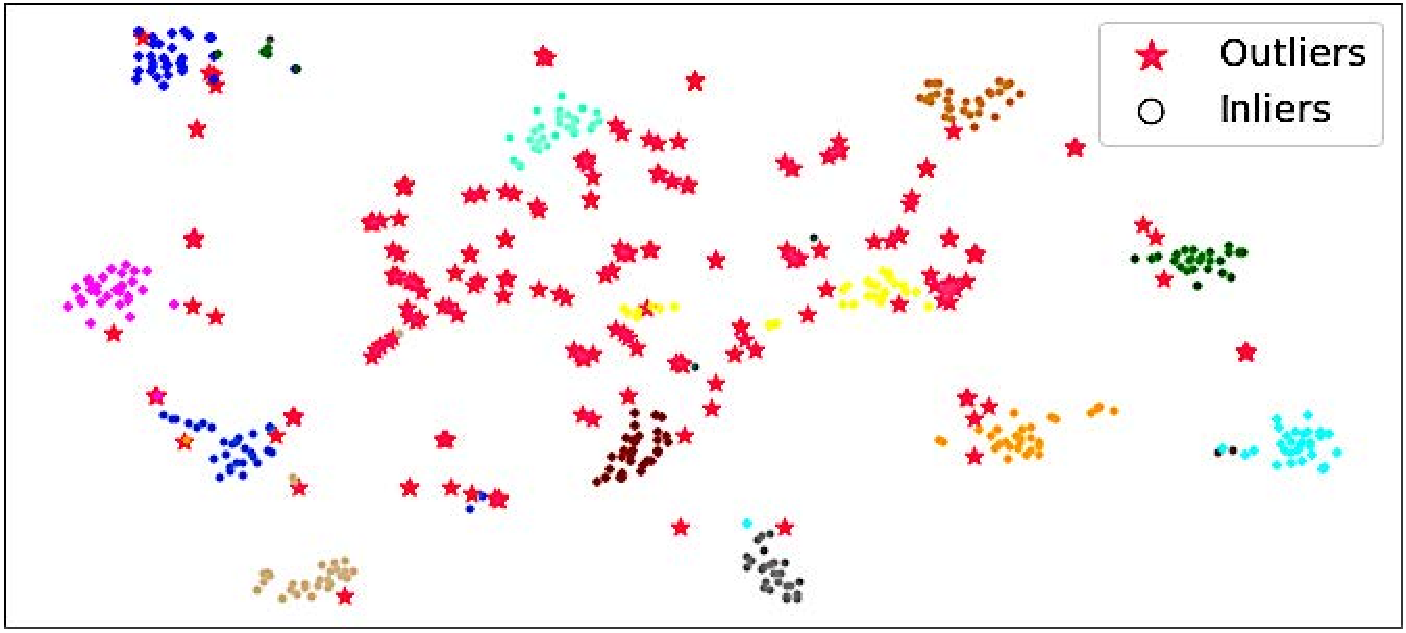
\includegraphics[width=.97\linewidth,height=0.152\textheight]{feat_base.pdf}
%   \caption{}
%   \label{fig:tsne_baseline}
\end{subfigure}
\begin{subfigure}{0.49\textwidth}
  \centering
  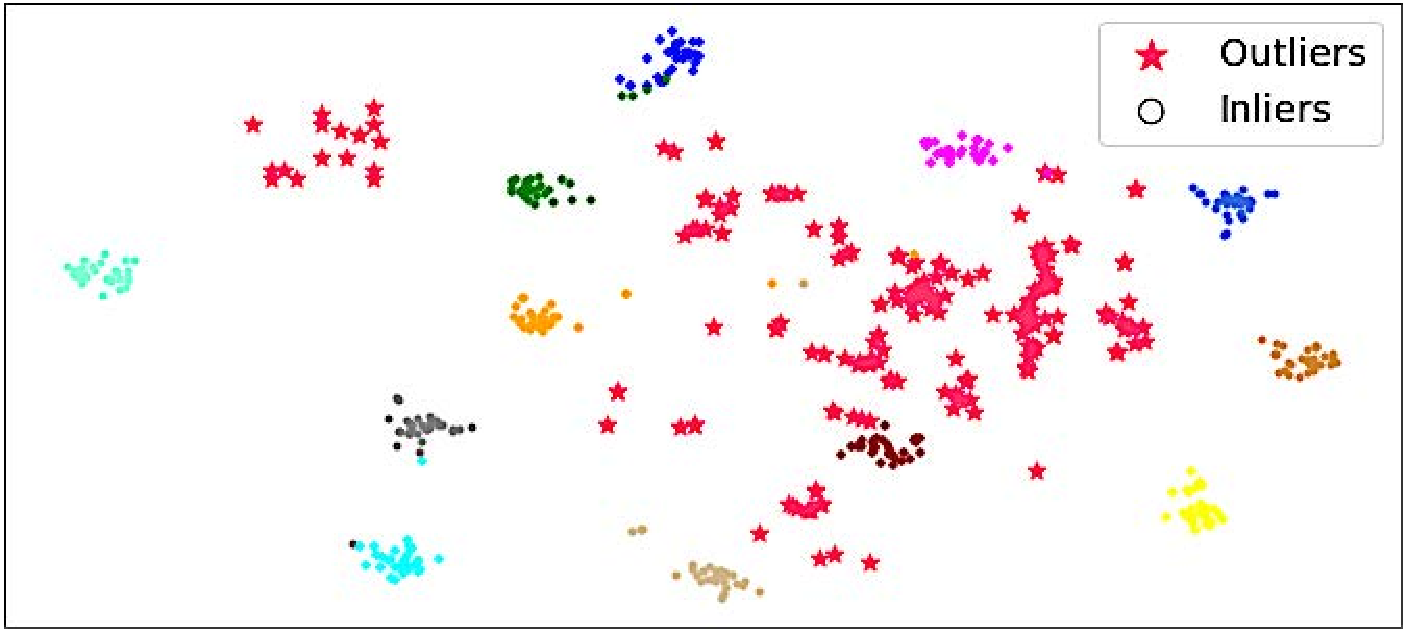
\includegraphics[width=.97\linewidth,height=0.152\textheight]{feat_visual.pdf}
%   \caption{}
%   \label{fig:tsne_ours}
\end{subfigure}
\vspace{-5pt}
\caption{t-SNE visualization of the learned embeddings of the test samples of CLINC150. Top: Previous $K$-way training; Bottom: Our proposed $(K+1)$-way training. Better view in color and enlarged.}
\label{fig:tsne}
\end{figure}